% \begin{figure}[h!] 
	\centering
	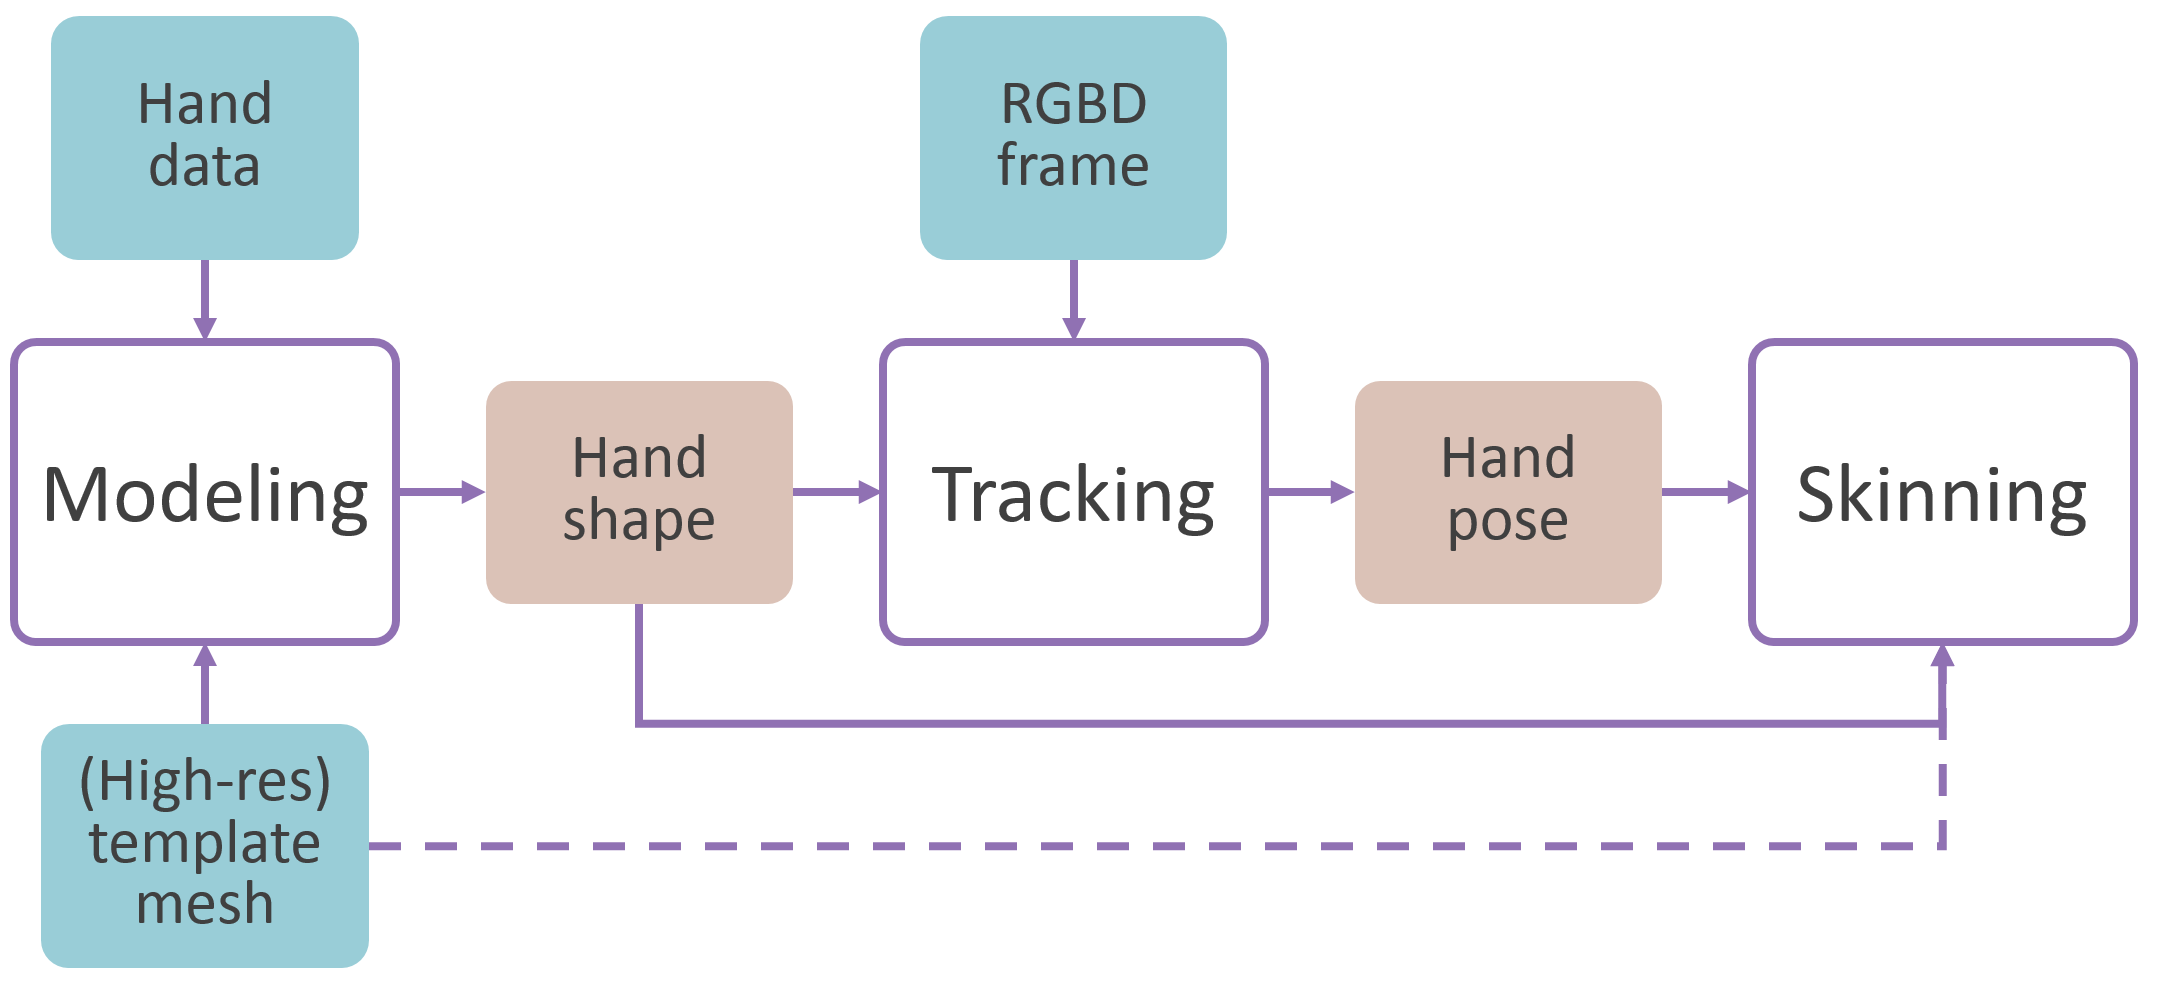
\includegraphics[width=0.5\textwidth]{fig/generic_pipeline}
	\caption{Generic pipeline for hand tracking. The input data that does not depend on the internal hand model representation is shown in blue, the representation-dependent components are shown in beige, and are listed in Table \ref{table:representation_dependent_components} for different representations.}
	\label{fig:generic_pipeline}
\end{figure} %<<< TO REMOVE!

However, in most consumer applications hand tracking is just a single components of a bigger pipeline (Figure \ref{fig:generic_pipeline}). Before tracking, a suitable hand model is obtained. Once the hand pose parameters are found, the tracking result is displayed by skinning the model. Both modeling and skinning tasks are not trivial.

\begin{figure}[h!] 
\centering
\hspace{-2em}
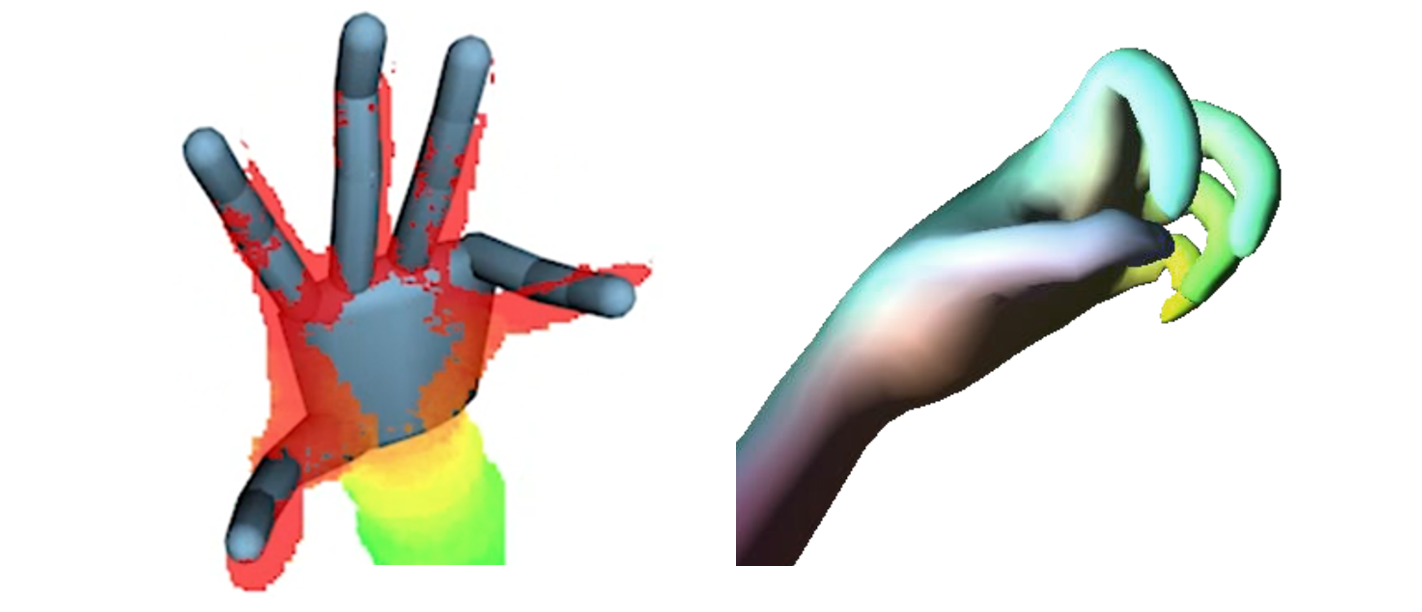
\includegraphics[width=0.5\textwidth]{fig/coarse_hand_model_and_lbs}
\caption{}.
\label{fig:coarse_hand_model_and_lbs}
\end{figure}

Especially if the hand model does not reflect all the degrees of freedom of a hand (Figure \ref{fig:coarse_hand_model_and_lbs}, left).

Each stage of the pipeline requires a hand model. There is several different hand model representations suggested by previous authors (see Figure \ref{fig:hand_model_representations}). Each representation is well suited for one of the stages, since it was used for the task on the first place. We argue that each representation also has weaknesses, which is why there exists a set of alternatives.

%--- OLD CONVOLUTION SURFACES TEXT
We suggest to use convolution surfaces representation of the hand model. Convolution surface is an implicit surface which is described by a control skeleton. The skeleton may consist of points, edges or polygons \cite{bloomenthal1991convolution}. In each vertex of the skeleton we define a radius. The radius in intermediate points is a linear combination of the radii at the neighboring vertices. Given the topology of the underlying skeleton, the model can be represented with convolution surface up to high precision \textcolor{mygray}{(find some theoretical estimates).} Next we present the arguments why convolution surfaces representation is suitable for all the stages of the pipeline.